\documentclass[12pt,a4paper]{article}

\usepackage{float} % use with [H] to anchor figures
\usepackage[table,xcdraw]{xcolor}
\usepackage[open,openlevel=1]{bookmark}
\usepackage{amsmath,fancyhdr}
\usepackage{graphicx}
\usepackage[ruled,vlined]{algorithm2e}
\usepackage{subcaption}
\setlength{\parindent}{0pt}
\hypersetup{pdfborder = {0 0 0}} % no colored links on table contents
\usepackage[top=1in, bottom=1in, left=1in, right=1in]{geometry}

\linespread{1.0}
\setlength{\parskip}{8pt plus2pt minus2pt}

\begin{document}



\title{Predicting Tesla's Stock Price\\
	\large ECS171 Fall 2021}
\author{Alvin Agana, Caitlin Brown, Tsung Chieh Chen, \\Aranza Cortes, Mckenzie Hochberg, Grant Koziol, Ryan Place, \\Clare Tran, Dingxian Wang, Stacy Zhu, Leon Zhuang}
\date{December 5, 2021}
\maketitle
\pagestyle{fancy}
\fancyhf{}
\tableofcontents
\newpage
\rhead{ECS 171 FQ 2021}
\lhead{Group 11 Final Report}



\section{Introduction}
The development of machine learning methods has allowed for more accurate and efficient prediction of stock prices and forecasting a company’s market value. Tesla, Inc, an American company founded in 2003, primarily focuses on the expansion of all-electric vehicles, clean energy generation and storage products [1]. Tesla went public in 2010 with an opening price of \$17 a share on the NASDAQ stock market and its IPO alone raised over \$226 million [6]. Through the application of machine learning methods, the goal is to design and execute predictive models to prognosticate future stock prices of Tesla by analyzing the daily stock prices of Tesla while also considering the attributes provided. Ideally, the results can be applied appropriately to maximize significant gains and assist financial institutions with market research. 

Since the stakes are large due to the financial crisis and scoring profits, it is significant that there must be a secure and accurate prediction of the values of the stocks [3]. There is a turnover of trading, approximately thousands of billions dollars, which effectively provokes individuals in making a profit. A share is more valuable the more it is conducted while on the other hand, it loses its value when put into a transaction in a low volume as it becomes less important for some traders [3]. The market can therefore result in profits or losses when one expects it to behave a certain way. That is where the problem of generating a reliable model in predicting stock prices comes in. When given a stock market history, the goal is to find out when the most appropriate time for buying or selling the share would be in order to generate profit. If it is possible to precisely predict the future trends of a stock, this would greatly reduce the financial risk and effectively minimize loss. 

Stock price prediction can be applied to the historical data of TESLA INC (TSLA) stock as an example for the following designed prediction algorithm. TSLA is a challenging stock to predict as the previous trends for the stock is not one of undeviating, rather it is constantly fluctuating due to external factors such as supply and demand. An example of this includes missed predictions in the second quarter of 2017. Due to this error, TSLA had lost over 5\% of the company stock price value which resulted in a loss worth \$12 billion [6]. In addition, Elon Musk, the CEO of Tesla, publicly posted on a popular social media application, Twitter, announcing that he had planned to make the company private when the stock price reaches \$420. Consequently, this resulted in an elevation of 10\% in TSLA’s stock price as investors were motivated to buy more shares before the supposed privatization announced by Musk [6]. 

As stock market predictions have the ability to significantly impact the global economy, it is important to understand how to analyze the volatility of the stock market. However, it turns out to be very difficult to predict the stock market as the rapidly changing state of it is too large to be captured in a model [1]. Even though there are these known difficulties involved with forecasting the stock market, this does not mean that there is no desire to develop a model that is reliable in doing so. In fact, it is actually the opposite in which there is a continuous desire to build and employ new approaches to tackle this problem in Artificial Intelligence, specifically Machine Learning [7]. 

\section{Literature Review}
Since the financial data of the real world is complicated, there were many limitations that early studies using statistical methods faced [2]. This was due to numerous statistical assumptions like normality and linearity. Therefore, some machine learning techniques that have the ability to capture non-linearity and complexity have been applied to predicting the stock market. These include artificial neural networks (ANN) and support vector machines (SVM). There have also been attempts on utilizing deep learning techniques in which deep belief network (DBN), convolution neural network (CNN), and recurrent neural network (RNN) are commonly used methodologies [2]. 

Developed by RNN, long short-term memory (LSTM) neural networks help forecast financial time series and are able to avoid long-term dependence issues as a result of its special storage unit structure [4]. LSTM is able to remember important events that occurred in the past, from many time steps ago, due to its memory [10]. As a result of this memory feature, RNN proves to be advantageous compared to the traditional ANN because of its ability to evoke temporal patterns in data. Although LSTM is commonly used in speech and image recognition due to its attention mechanism, it is rarely used in finance because of its high noise-to-signal ratio which makes models difficult to predict future prices as they are unable to identify patterns in a dataset. 

Deep learning models have promising results as they can significantly improve the accuracy. Although it was explored that RNN models like LSTM could perform better than ANN, there have been many approaches using ANN to predict stock prices. One application of this model used Nifty stock index dataset and was able to achieve an accuracy of 96\% with the average accuracy over all the cases as 88\% [9]. In this ANN approach, there are customizable parameters and various activation functions are executed that have the option for cross validation sets as well. 

There is also another proposed system that uses both Regression and Classification in order to predict stock prices. The system will predict the closing price of stock of a company in regression while with classification, the system will predict if the closing price of the stock will increase or decrease the following day [5]. Some regression models that are applied include: simple linear regression, polynomial regression, and support vector regression. The classification algorithms to determine whether the stock will go high or low the next day include: SVM, logistic regression, and Naive Bayes. The accuracy obtained from the models depend largely on the input dataset and does not indicate which algorithm or model provides the best results when used. 

To conclude this section, there have been previous findings that go beyond the typical models for regression that are usually implemented in forecasting stock prices. In order to approach the problem of predicting stock prices, regression analysis methods will not solely be used in this project but also methods like LSTM and SVM. This is due to their promising results in modeling complex systems and capturing non-linearity. The results from previous research demonstrate how there are other machine learning techniques that one may not initially think fits the problem statement but actually could produce favorable results. Since the stock market is known for being volatile, nonlinear, and dynamic, it is important to look into analytic techniques being explored in order to detect these trends.

\section{Dataset Description}
The dataset provides information about Tesla stock data from June 29, 2010 to October 8, 2021 (Figure 1). It consists of 2841 observations in which the data is available on a daily basis. The currency of the data provided is all in terms of USD. 

Within the TSLA.csv data, there are seven attributes: Date, Open, High, Low, Close, Adj Close, and Volume. Date is formatted as yyyy-mm-dd and is provided on a daily level, taking into account that there are no regular trading hours for stocks on the weekends. The Open attribute is the Tesla stock price at the start of trading day. Similarly, the Close attribute is the stock price at the end of the trading day. The Adj Close attribute stands for “adjusted close” which is the closing price after adjustments to reflect the stock’s value after taking corporate actions into consideration. Adj Close factors in corporate actions including stock splits, dividends, and right offerings. The High attribute tells us what the maximum price is on that trading day. Meanwhile, the Low attribute is the minimum price on that trading day. The Volume is the amount of Tesla stocks traded on that day and is represented by a positive integer number and the rest of the attributes are all decimal numbers in USD. 

Minimal data cleaning was necessary for this dataset as there were no null or missing values found. When conducting a heatmap, we found the lowest correlation to be between Volume and all other attributes and was therefore dropped from the dataset. The Date attribute was converted from a categorical attribute to a float in which the year is a whole number, followed by the month and day as a decimal. There were 513 outliers found in this dataset, but were not removed because once removed, our models were not able to quite capture the complexity of the dataset and nature of the stock market. 

\begin{figure}[h]
\caption{Tesla Stock Price 2010-2021}
\centering
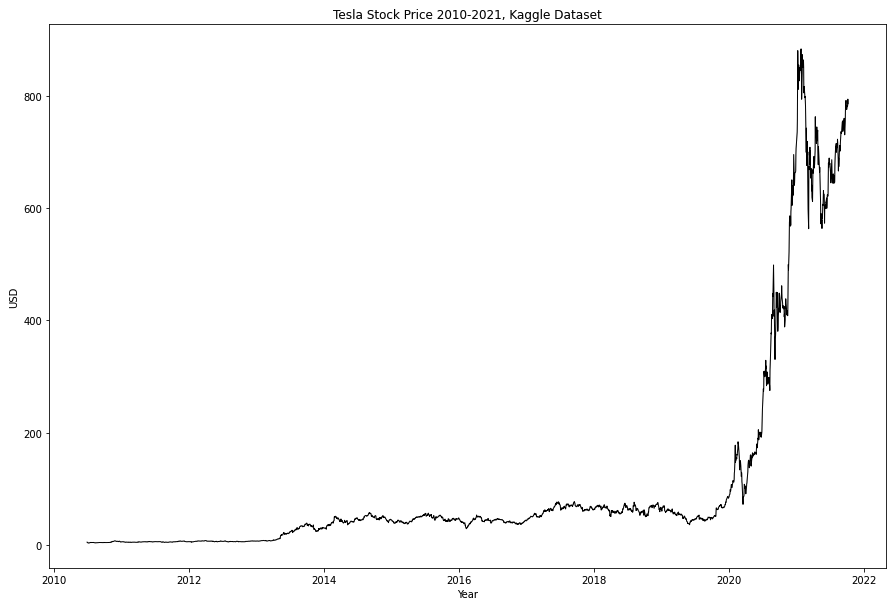
\includegraphics[width=3in]{./Figures/TSLA.png}
\end{figure}
\section{Methods}
\subsection{Linear Regression}
Linear regression is a statistical technique for modeling a relationship between one or more explanatory variables and a scalar response. In this case, we decided to do a simple linear regression and only use one explanatory variable: the date. Naturally, linear regression is a good approach for modeling linear relationships. However, due to TSLA stock data non-linearity, this was a poor choice of model as it was severely under-fitting.

\subsection{Polynomial Regression}
Polynomial regression is a technique for modeling the relationship between the explanatory variable(s) and the dependent variable using an nth degree polynomial. It is a slightly better choice for our problem because the TSLA stock price is not linearly related to the date. The constructed model fits polynomials of degree 2, 3, 4, 10, 20, 25, 50, and 100. To evaluate the results we plotted the resulting curves and looked at both the training and testing mean squared error (MSE).

\subsection{Support Vector Regression}
Support vector regression (SVR) is a type of model that uses Support Vector Machines (SVMs) in regression problems. While SVMs are usually used in classification problems, SVR is also a strong algorithm for regression problems. To prepare the data to fit the model, we use all the columns in TSLA stock data excluding “Close” and “Adj Close” in the sample vectors, and values of both samples and targets are used after scaling. 
Next, grid search was applied to tune the hyper-parameters. Based on the performance of a series of combinations, we choose to use RBF (radial basis function) as the kernel, 1000 as the regularization parameter (C), and 0.001 as the kernel coefficient ($\gamma$). An SVR model was then built with the hyper-parameters chosen above. 

\subsection{Long Short-Term Memory}
Long short-term memory models are variations of recurrent neural networks, a class of artificial neural networks where connections between nodes form along a temporal sequence. This makes them an algorithm of choice for making time series predictions. As such, a first step after scaling the prices to values within the range [0,1] is to tag each stock price instance with a timestamp. We assign a timestamp relative to the rest of the dataset rather than using the datetime instance in the dataframe.

We then build an LSTM model using Keras with 3 layers of 50 nodes and an output layer with one dense node. We use Adam optimization with a learning rate of 0.01, a batch size of 64, mean squared error as our loss function, and run for 100 epochs. For computational efficiency, we implement early stopping if the MSE between our predicted and observed results falls under a certain threshold for 10 or more epochs.

Next, we use Bayesian Optimization to tune the hyper-parameters of our model. We chose Bayesian Optimization for this because, like LSTM, this method of hyper-parameter tuning works well for large datasets, as well as datasets that are complex and expensive to evaluate. The hyper-parameters we chose to tune were the number of units, i.e. the number of nodes per layer, and the learning rate for the optimization function. To do this, we use BayesianOptimization from keras\_tuners. First we define a function with a set of hyperparameters variables as a parameter. The number of units is varied using a scalable approach, testing numbers from 8 to 64 with a step size of 8. The learning rate is given a set of values to search through ([0.01, 0.001, 0.0001]). This function is passed to keras to search for the best hyper-parameters. We defined the “best” hyper-parameters as those with the lowest MSE value. After a set of optimal hyper-parameters are found, we retrain the model using these hyper-parameters. 

\section{Results}
This project so far has applied four different machine learning methods to the dataset: linear regression, polynomial regression, long short-term memory (LSTM), and support vector regression (SVR).

\subsection{Linear Regression}
Even though we knew that the linear regression would not provide a good fit for our model, we still decided to create the model to help explore our data and display a general correlation between the variables. The first problem we ran into is that scikit-learn did not like how our date was formatted (dd/mm/yyyy), so we had to use the pandas function “to\_datetime” to convert it into an acceptable format. 

With this problem solved, we created a linear model (Figure 2) using scikit-learn using “date” as the independent variable and “close” as the target. We also used an 80/20 train/test split.

\begin{figure}[h]
\caption{Linear Regression Model}
\centering
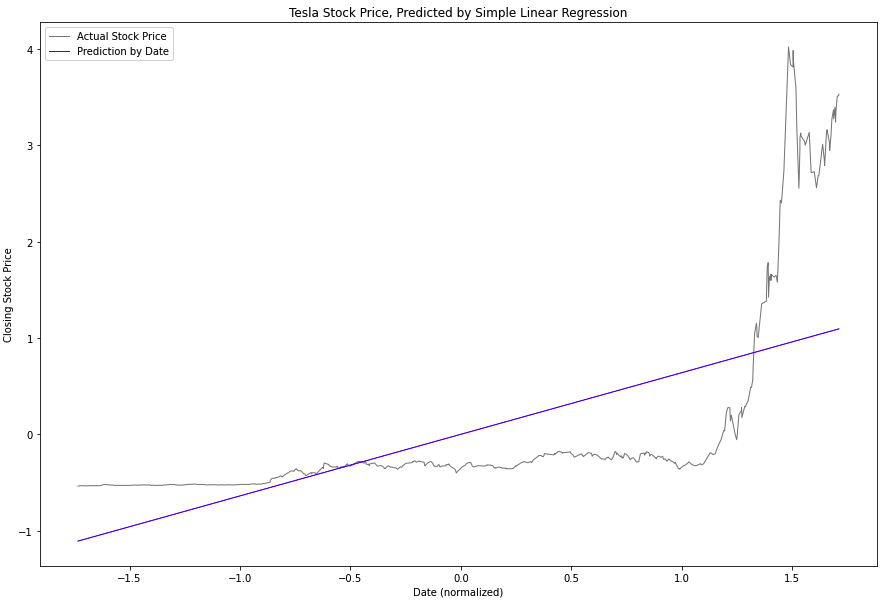
\includegraphics[width=3in]{./Figures/LinearRegression.png}
\end{figure}

This model had a mean squared error (MSE) of .5891. As our group had assumed, the linear model showed clear signs of under-fitting and did not capture the complexity in the data. However, this graph allows us to better understand our data. As we can see from 2010-2020, TSLA stock price did not grow but stayed stagnant and eventually experienced a heavy upward trend that remains till today.


\subsection{Polynomial Regression}
Due to the severity of under-fitting with linear regression, we decided to trial with polynomial regression to achieve a better result. Our first model was almost the same as the linear model, using the date as the independent variable and an 80/20\% train/test split, but we also used several different degrees (Figure 3). 

\begin{figure}[h]
\caption{Polynomial Regression Model: Date}
\centering
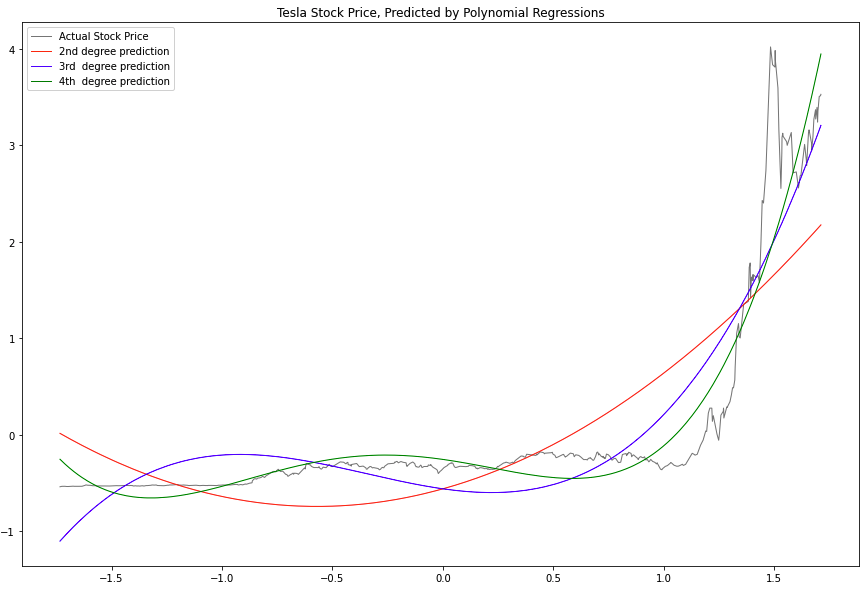
\includegraphics[width=3in]{./Figures/PolyRegression1.png}
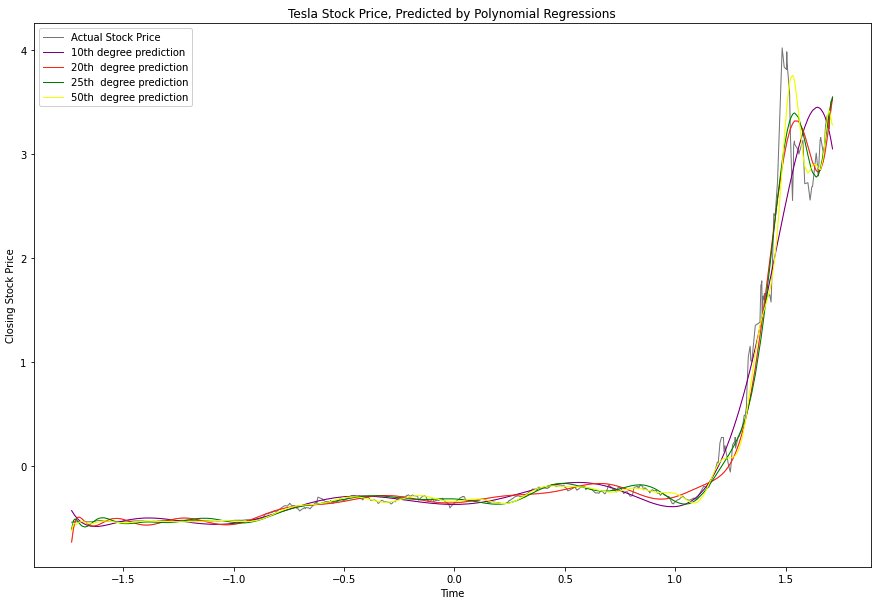
\includegraphics[width=3in]{./Figures/PolyRegression2.png}
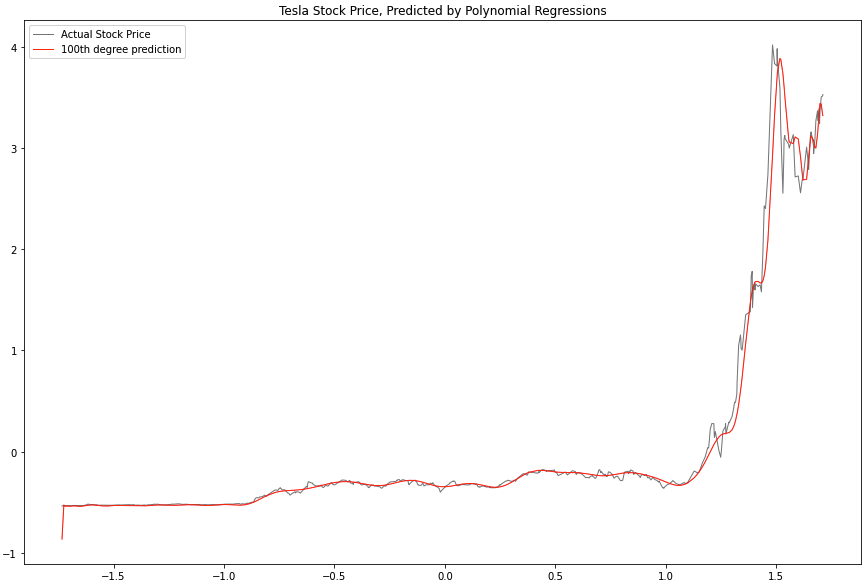
\includegraphics[width=3in]{./Figures/PolyRegression3.png}
\end{figure}

As expected, under-fitting was not an issue here, these new models are capturing the complexity of the data. Between all the models, 25th degree (green) created the optimum outcome as it captured most of the complexity without signs of over-fitting and ended with an MSE of .00119.
With this done, we decided to explore some other options for our independent variable. We trained an extremely similar model (Figure 4), but decided to use the opening price as the independent variable.

\begin{figure}[h]
\caption{Polynomial Regression Model: Opening Price}
\centering
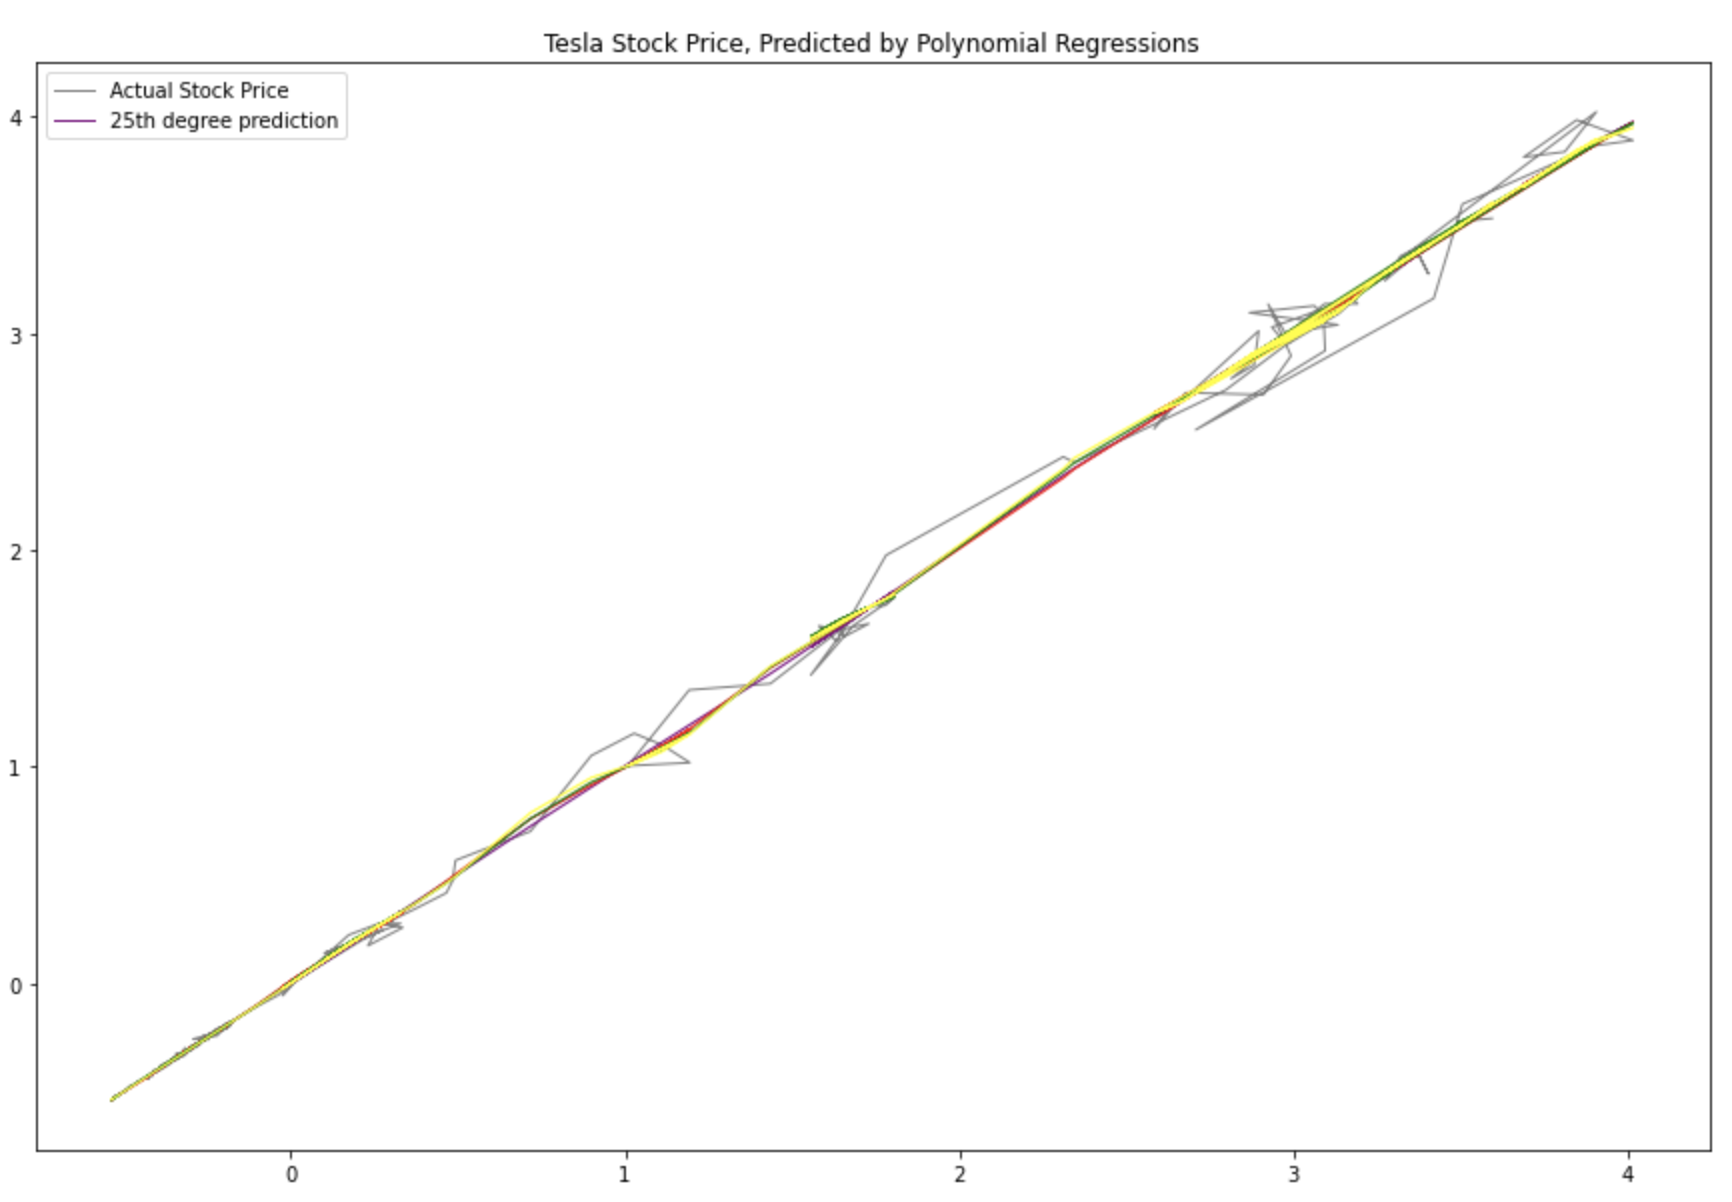
\includegraphics[width=3in]{./Figures/PolyRegression4.png}
\end{figure}

The relationship between opening price and closing price appears to be linear and the MSE is very low, at around .001. The training and testing MSEs for all the polynomial models (with the date as the independent variable) we fit are summarized in Table 1.

\begin{table}[h]
\caption{Polynomial Regression Metrics}
\centering
\begin{tabular}{ccc}
\hline
\hline
Degree & Training MSE & Testing MSE \\ \hline
2      & 0.33918      & 0.32282     \\
3      & 0.16516      & 0.14752     \\
4      & 0.09014      & 0.08427     \\
10     & 0.03856      & 0.03689     \\
20     & 0.01632      & 0.01834     \\
25     & 0.01412      & 0.01651     \\
50     & 0.00912      & 0.01687     \\
100    & 0.00517      & 0.01610     \\ \hline
\hline
\end{tabular}
\end{table}

\subsection{Support Vector Regression}
This model, with the chosen hyper-parameters, had impressive results. We split the dataset with the same strategy of 80/20\% for train and test sets, and the MSE is as low as .0008, which is the lowest one among all the models we trained. Figure 5 shows the model’s prediction on the test data. 

\begin{figure}[h]
\caption{Support Vector Regression Model}
\centering
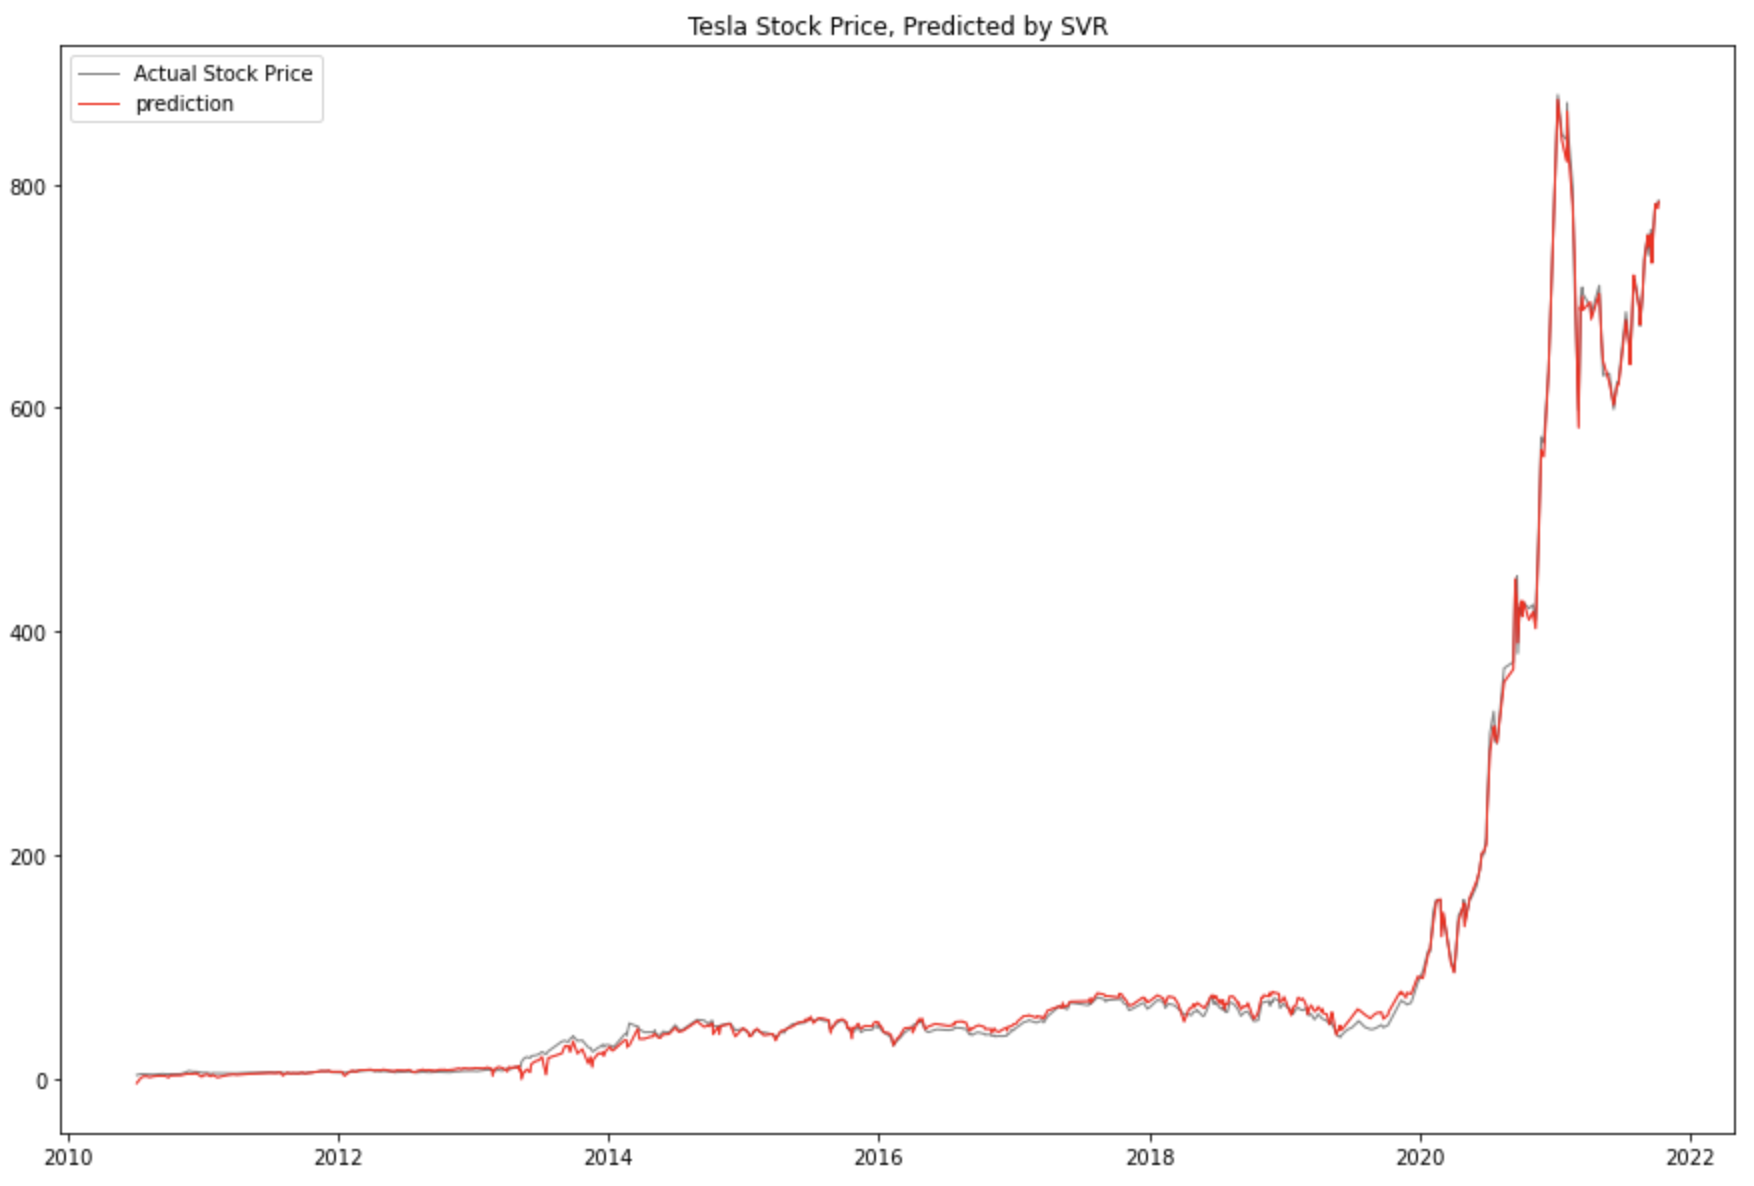
\includegraphics[width=3in]{./Figures/SVM.png}
\end{figure}

In the graph above, the red line, representing the prediction value, always approaches to or covers the grey line that represents the true value. The accuracy of the prediction is also shown by how the predicted values are close to the steep changes of real prices after 2020. However, the performance of the SVR model also shows a great chance of over-fitting.

\subsection{Long Short-Term Memory}
We fit our LSTM model twice — before and after hyper-parameter tuning. Before tuning, it stopped early at 74 of 100 epochs with a training MSE (loss) of 4.7977e-06 and a testing MSE (val\_loss) of 0.0165. Figure 6 illustrates our model loss over epochs, and the accuracy of the model’s predictions compared to the observed stock price.

After hyper-parameter tuning using Bayesian optimization, training the model stopped early at epoch 57 out of 100 with a training MSE (loss) of 5.2846e-06 and a testing MSE (val\_loss) of 0.0250. Though these loss values are slightly higher than those found before hyper-parameter tuning, this model significantly decreased training time.

\begin{figure}[h]
\centering
\caption{LSTM results before (above) and after (below) hyper-parameter tuning}
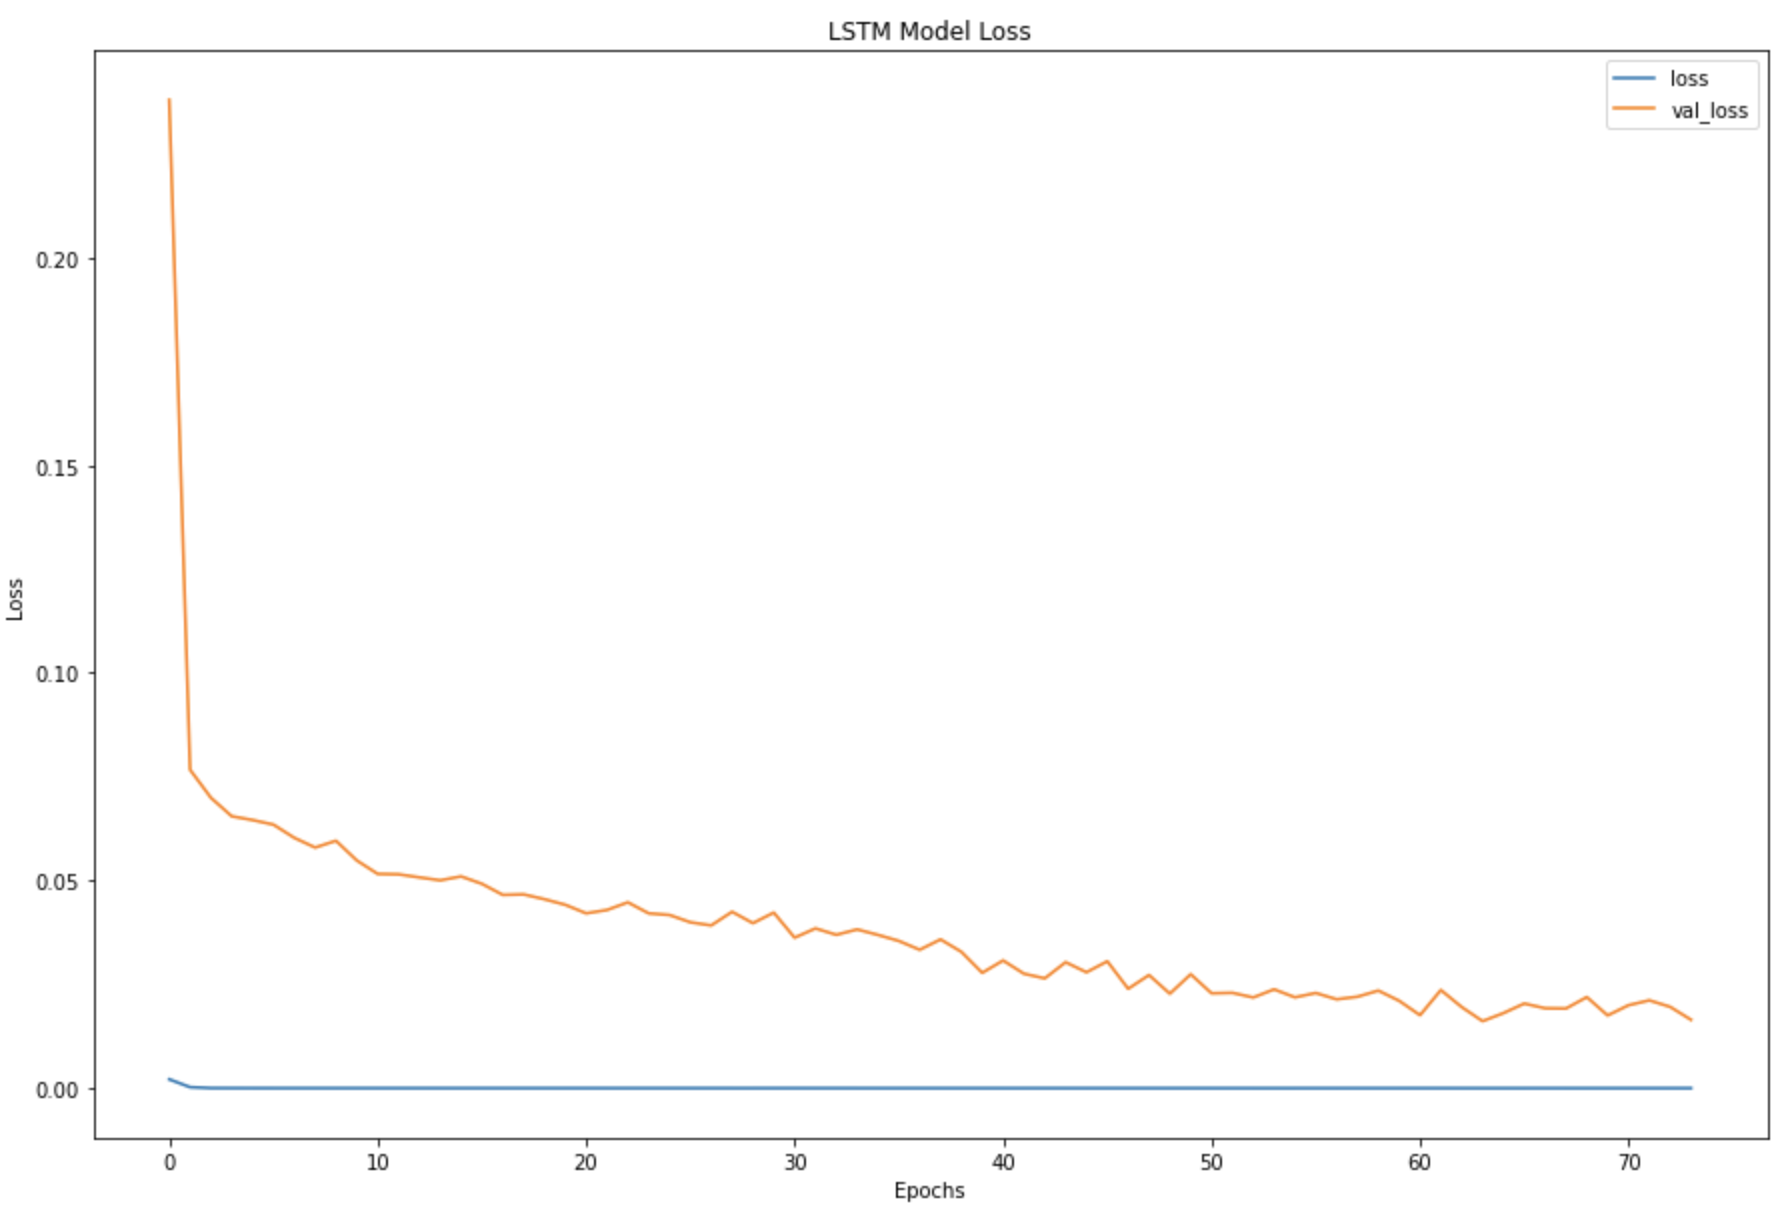
\includegraphics[width=2.5in]{./Figures/LSTM1.png}
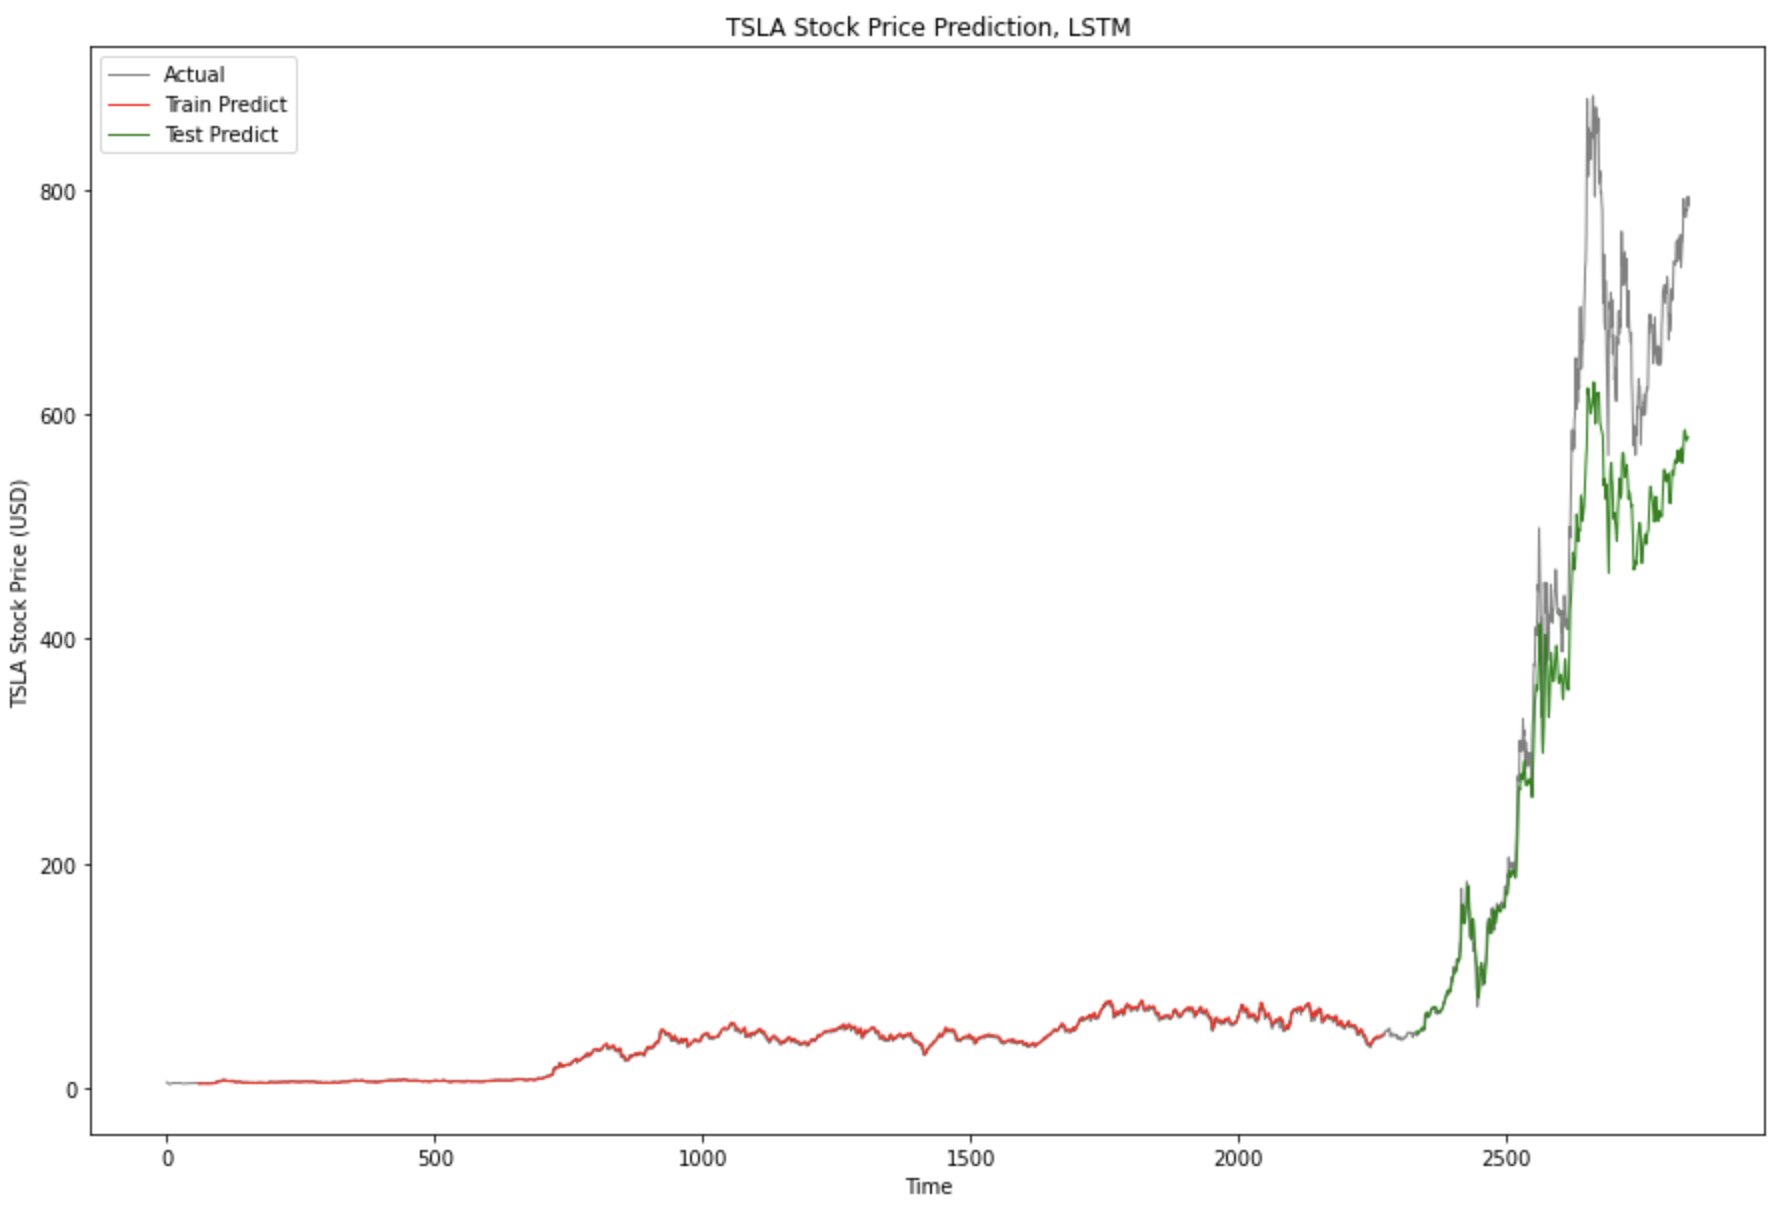
\includegraphics[width=2.5in]{./Figures/LSTM2.png}
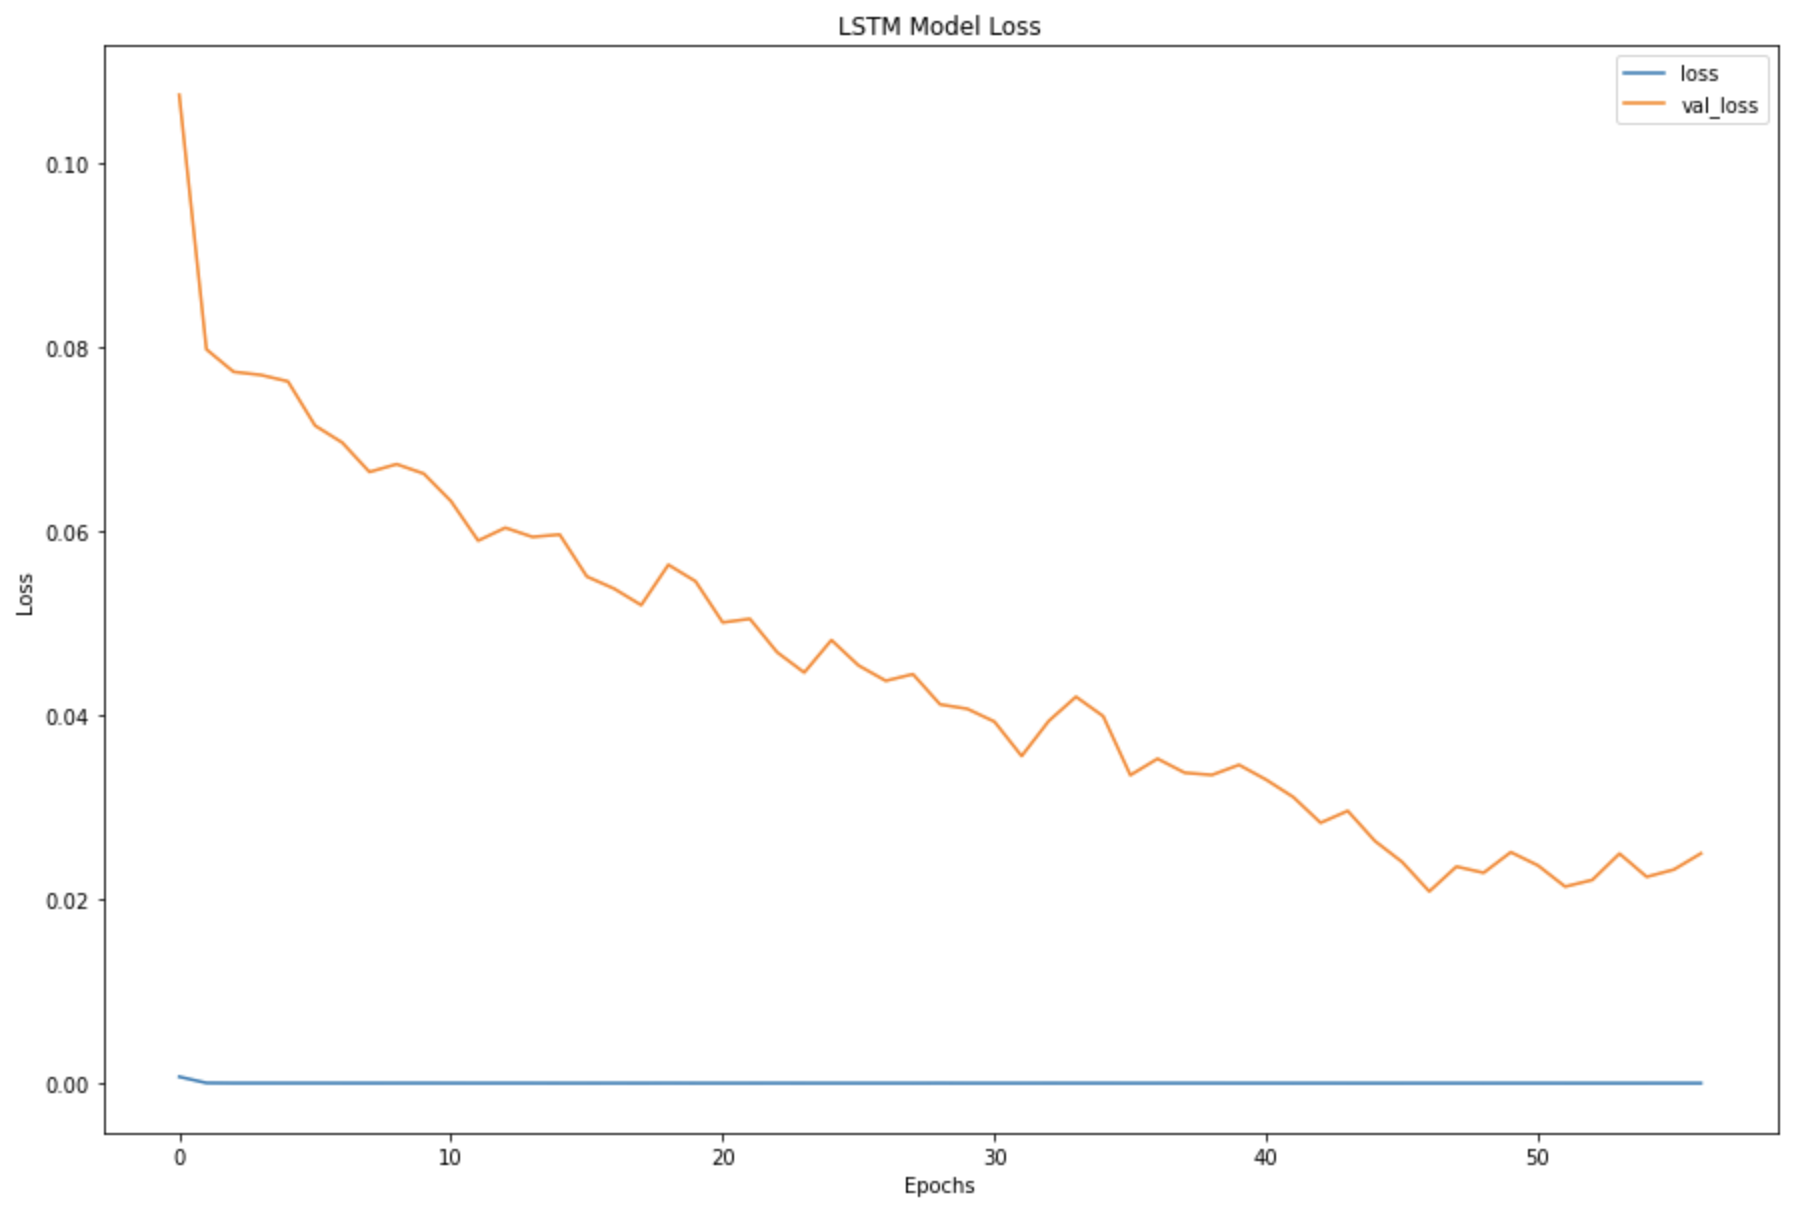
\includegraphics[width=2.5in]{./Figures/LSTM3.png}
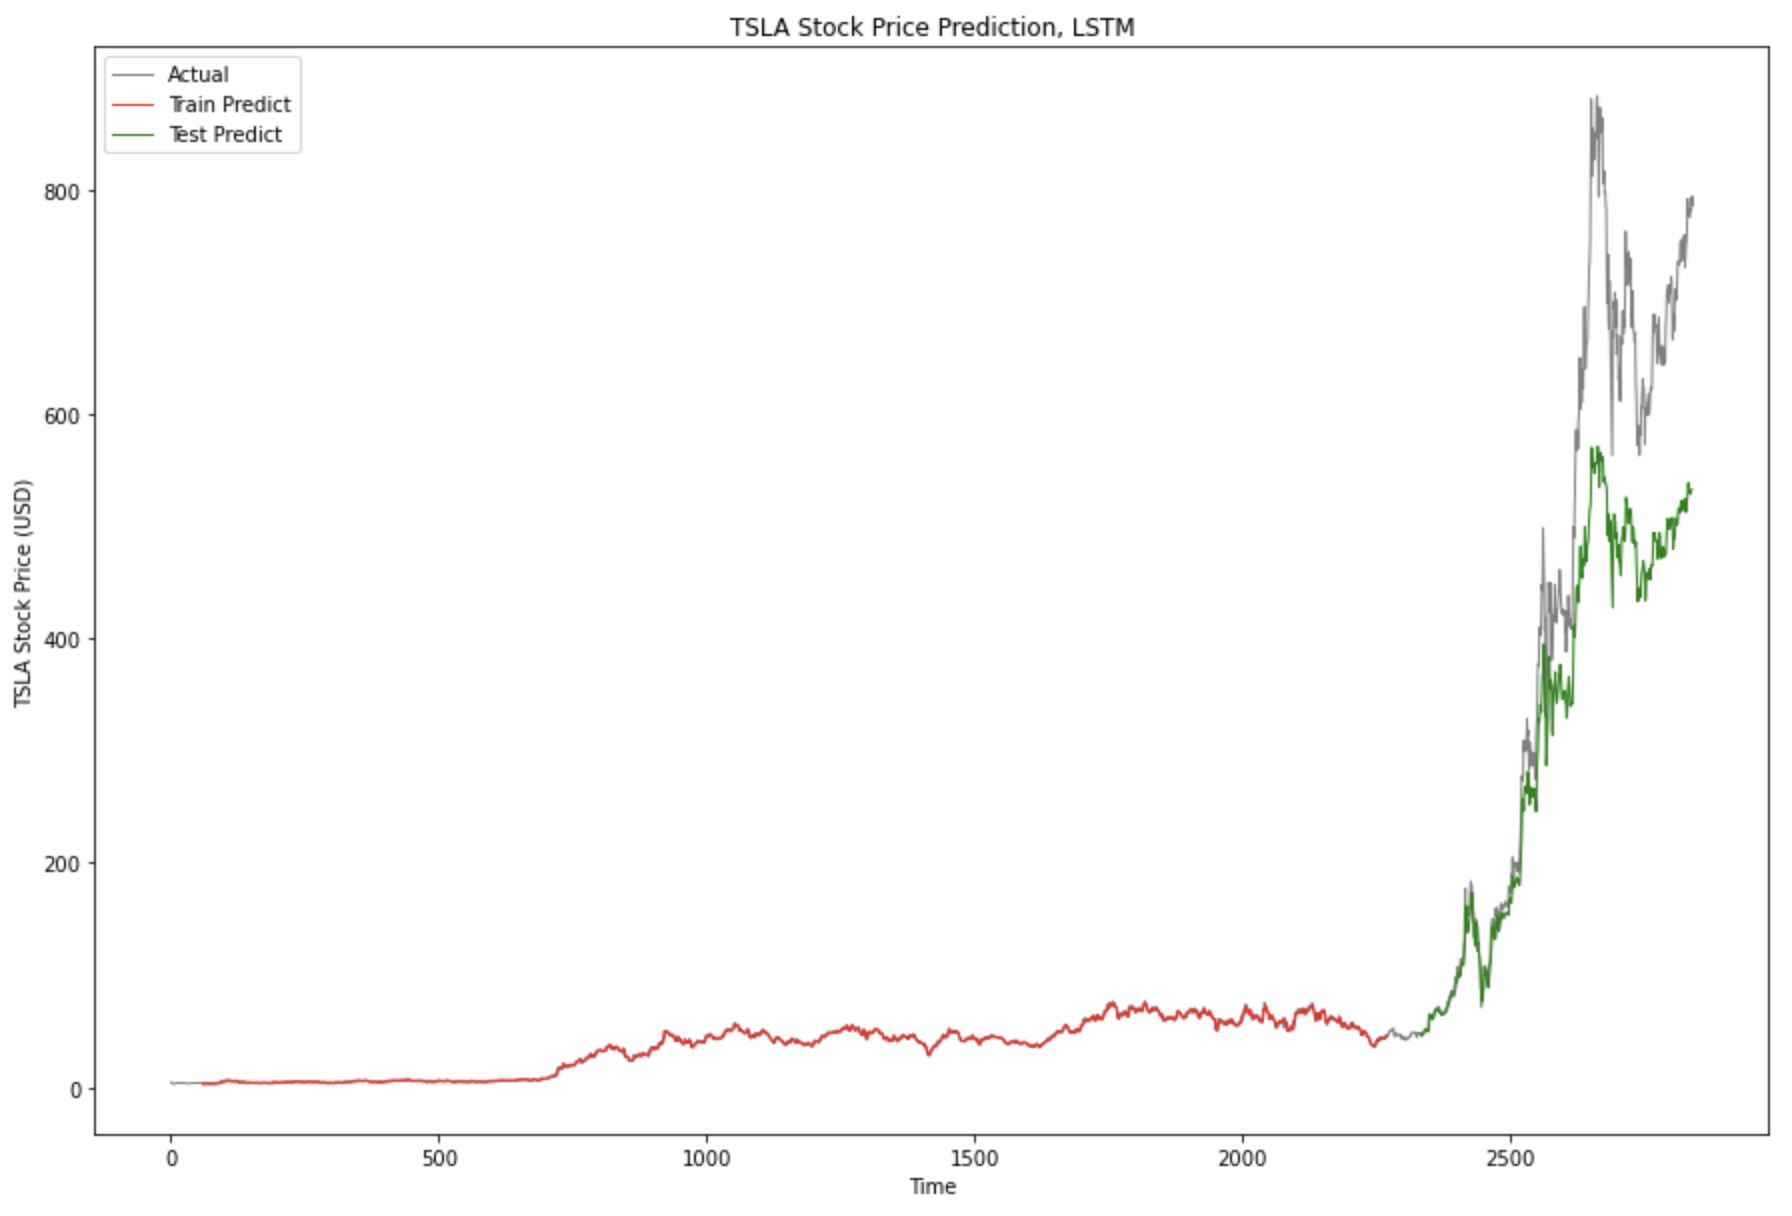
\includegraphics[width=2.5in]{./Figures/LSTM4.png}
\end{figure}

\section{Conclusion}
The prediction of the stock market and its value is a classic and challenging topic in the field of Machine Learning. Although stock prices are affected by many kinds of real world factors that we are unable to easily include in a Machine Learning model, the performance of our models is acceptable for stock price prediction when applied to the existing historical data. We believe that the price prediction made by certain Machine Learning models can be used as guidance material for decision making in the real stock market. 

After consideration of all the models, the polynomial model with date as the independent variable, closing price as the target, and degree 25 resulted in the best outcome. This model has an MSE of .00119 and could accurately predict historical data without signs of over-fitting. While this model may struggle with predicting future stock prices, it achieved much better results than the linear model, which did not capture the complexity, and the SVM and LSTM, which both showed signs of over-fitting. As such, we decided to use the polynomial model for our project demo and this report.

As for our future works, we are hoping to implement sentiment analysis into our models. This is a technique that allows us to analyze Tesla’s social media activity and use that activity as an additional attribute for our models. This extra attribute means that we can predict Tesla’s stock prices based on real world factors and will significantly increase our accuracy in predicting future stock prices.

\section*{References}
\begin{enumerate}
    \item Atsalakis, G. S., \& Valavanis, K. P. (2009). Surveying stock market forecasting techniques – Part II: Soft computing methods. Expert Systems with Applications, 36(3, Part 2), 5932–5941. \url{https://doi.org/10.1016/j.eswa.2008.07.006}
    \item Chung, H., \& Shin, K. (2018). Genetic Algorithm-Optimized Long Short-Term Memory Network for Stock Market Prediction. Sustainability, 10(10), 3765. MDPI AG. Retrieved from \url{https://dx.doi.org/10.3390/su10103765 }
    \item Iacomin, R. (2015). Stock market prediction. 2015 19th International Conference on System Theory, Control and Computing (ICSTCC), 200–205. \url{https://doi.org/10.1109/ICSTCC.2015.7321293}
    \item Qiu J, Wang B, Zhou C (2020). Forecasting stock prices with long-short term memory neural network based on attention mechanism. PLoS ONE 15(1): e0227222.  \url{https://doi.org/10.1371/journal.pone.0227222}
    \item Ravikumar, S. \& Saraf, P. (2020), "Prediction of Stock Prices using Machine Learning (Regression, Classification) Algorithms," 2020 International Conference for Emerging Technology (INCET), 2020, pp. 1-5, doi: 10.1109/INCET49848.2020.
    9154061.
    \item Reed, E. (2020, February 4). History of Tesla: Timeline and facts. TheStreet.\url{https://www.thestreet.com/technology/history-of-tesla-15088992}
    \item Tay, F. E. H., \& Cao, L. (2001). Application of support vector machines in financial time series forecasting. Omega, 29(4), 309–317.  \url{https://doi.org/10.1016/S0305-0483(01)00026-3}
    \item Tesla (n.d.). About Tesla. Retrieved October 27, 2021 from \url{https://www.tesla.com/about }
    \item Verma, R., Choure, P., and Singh, U. (2017), "Neural networks through stock market data prediction," 2017 International conference of Electronics, Communication and Aerospace Technology (ICECA), 2017, pp. 514-519, doi: 10.1109/ICECA.2017.8
    212717.
    \item Zhang, Y., Chu, G., \& Shen, D. (2021). The role of investor attention in predicting stock prices: The long short-term memory networks perspective. Finance Research Letters, 38, 101484.  \url{https://doi.org/10.1016/j.frl.2020.101484}
\end{enumerate}

\appendix
\section{Appendix}

\subsection{GitHub}

Here is the URL for our GitHub repository:\\

\url{https://github.com/Diean233/ECS171-Project}

\end{document}
\end{document}